% Provenance (never printed): cycle 2 "Questionner l'espace et le temps ---
% se situer dans l'espace": representations of familiar spaces (plans), "lire
% des plans, se reperer sur des cartes. Elements constitutifs d'une carte :
% titre, echelle, orientation, legende"; see sources/book1/PROVENANCE.md.
% Book 1, grade 2, chapter 2. Sync 1: "scale" is owned here; "cardinal
% directions" is the physics series' term (prose only); "compass rose" here.
\chapter{Do desenho ao mapa}\label{ch:g2:drawing-to-map}

Um pombo voa por cima da escola. O que ele vê? Nem as portas da frente,
nem as janelas, nem o rosto das crianças: lá de cima, ele só vê a parte de
cima das coisas. Os telhados dos prédios são retângulos cinzentos. O pátio
é uma grande forma vazia com algumas copas de árvore redondas. Os caminhos
são linhas finas. O pombo vê a escola de cima --- do jeito que um \omterm{def:g2:drawing-to-map:map}{mapa} a mostra.

\begin{omfigure}
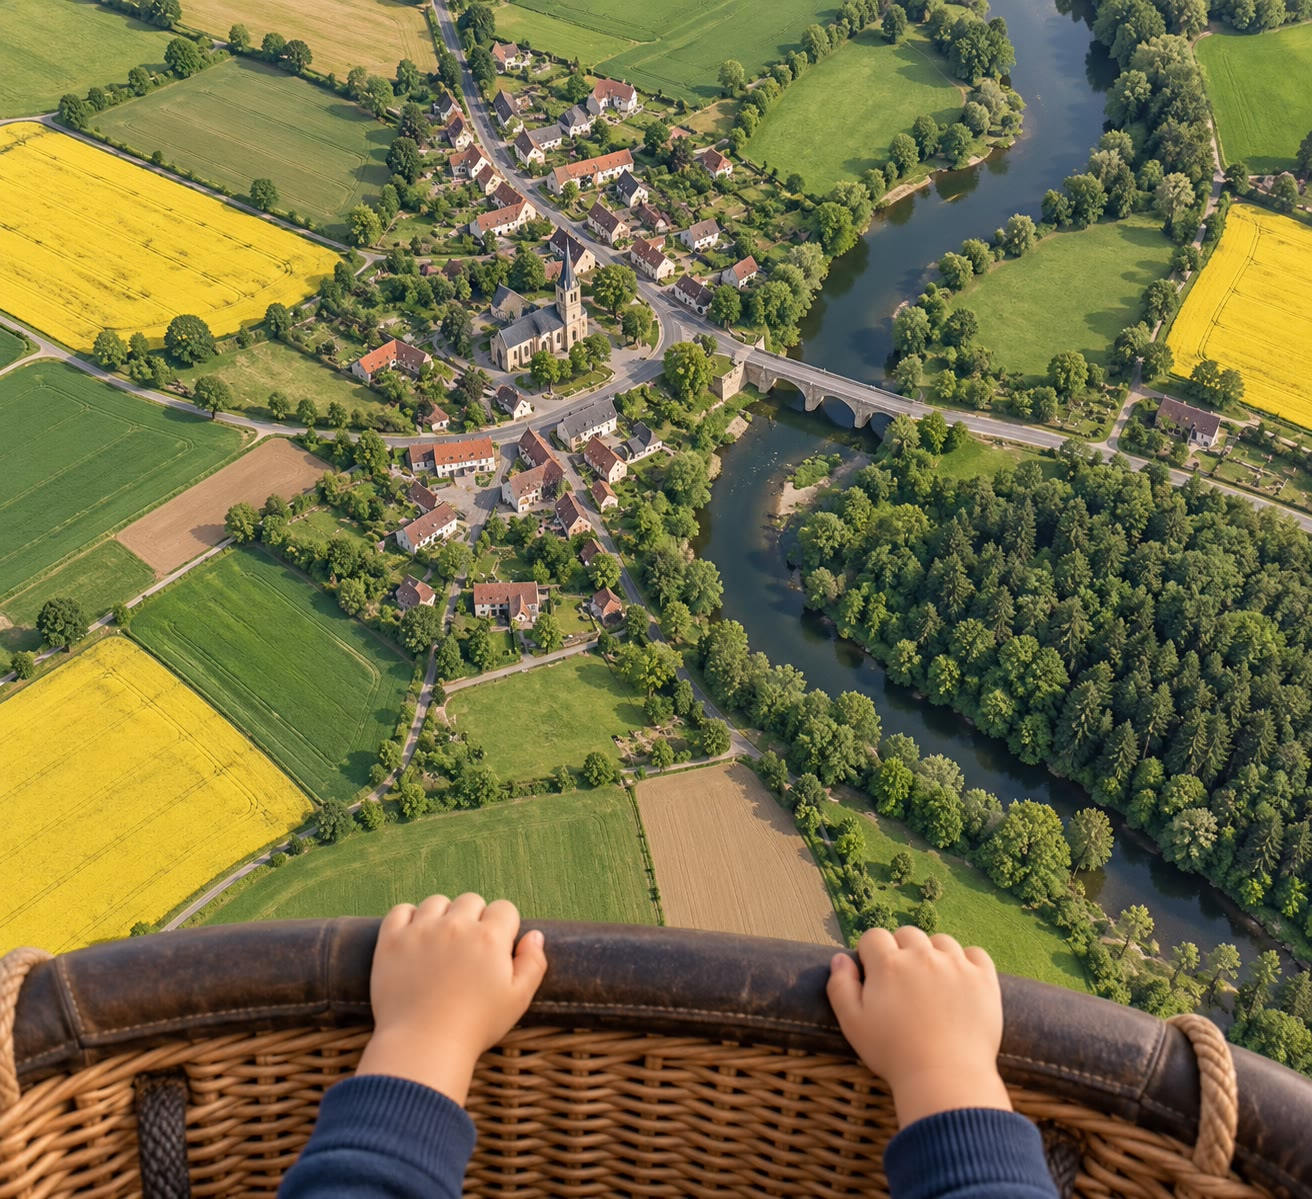
\includegraphics[width=0.62\linewidth]{images/book1/ai/g2-balloon-view.jpg}

{\small O campo visto de um balão: plantações, uma vila, uma estrada, um \omterm{def:g1:landscapes-around-us:water}{rio}
e a sua ponte, tudo visto de cima.}
\end{omfigure}

\section{Visto de lado, visto de cima}

Coloque alguns blocos de brinquedo sobre uma mesa. Olhe para eles de lado:
você vê a altura deles, e os que estão atrás ficam escondidos pelos da
frente. Agora fique de pé e olhe para eles de cima: você não vê mais a
altura de cada um, mas vê exatamente onde cada um está e a distância entre eles.

\begin{omfigure}
\begin{tikzpicture}[x=1cm, y=1cm, font=\small]
  % side view
  \begin{scope}
    \draw[black!50] (-0.2,0) -- (4.6,0);
    \fill[red!55, draw=black!60] (0.2,0) rectangle (1.2,1.6);
    \fill[ocBlue!55, draw=black!60] (1.6,0) rectangle (3.0,0.8);
    \fill[yellow!70, draw=black!60] (3.4,0) -- (3.9,1.1) -- (4.4,0) -- cycle;
    \node at (2.2,-0.5) {visto de lado};
  \end{scope}
  % from above
  \begin{scope}[shift={(6.4,0)}]
    \draw[black!30, fill=black!3] (-0.2,-0.1) rectangle (4.6,2.3);
    \fill[red!55, draw=black!60] (0.2,0.4) rectangle (1.2,1.4);
    \fill[ocBlue!55, draw=black!60] (1.6,1.0) rectangle (3.0,2.0);
    \fill[yellow!70, draw=black!60] (3.9,0.75) circle (0.5);
    \node at (2.2,-0.5) {visto de cima};
  \end{scope}
\end{tikzpicture}

{\small Três blocos sobre uma mesa: um bloco vermelho alto, um bloco azul
achatado e um cone amarelo. Visto de cima, o cone é um círculo e o bloco
alto é um quadrado.}
\label{fig:g2:drawing-to-map:blocks}
\end{omfigure}

\begin{definition}[Planta]\label{def:g2:drawing-to-map:plan}
Uma \emph{planta}\index{planta} é um desenho de um lugar pequeno --- um
quarto, uma casa, uma escola, um jardim --- visto bem de cima, desenhado
menor do que é na realidade, mas com cada parte no seu lugar certo.
\end{definition}

\section{Desenhar menor: a escala}

Uma sala de aula é grande demais para ser desenhada numa folha de papel
do tamanho que é. Nós a desenhamos menor --- mas cada parte tem de ficar
menor do mesmo jeito, senão a \omterm{def:g2:drawing-to-map:plan}{planta} engana. O jeito mais fácil é usar papel
quadriculado: um quadradinho do papel representa um metro da sala de aula.

\begin{definition}[Escala]\label{def:g2:drawing-to-map:scale}
A \emph{escala}\index{escala} de uma \omterm{def:g2:drawing-to-map:plan}{planta} ou de um \omterm{def:g2:drawing-to-map:map}{mapa} diz quanto o
desenho é menor que o lugar real: que distância no chão um comprimento do
desenho representa. Por exemplo: \emph{1 quadradinho representa 1 metro}.
\end{definition}

\begin{omfigure}
\begin{tikzpicture}[x=0.75cm, y=0.75cm, font=\scriptsize]
  \draw[black!15] (0,0) grid (10,8);
  \draw[black, line width=1.6pt] (0,0) rectangle (10,8);
  % board on the north wall
  \fill[black!70] (3,7.8) rectangle (7,8);
  % teacher's desk
  \fill[brown!50, draw=black!70] (4,6) rectangle (6,7);
  % pupils' desks: 3 rows of 3
  \foreach \x in {1,4,7} \foreach \y in {1,2.5,4}
    \fill[orange!45, draw=black!70] (\x,\y) rectangle ++(2,1);
  % cupboard
  \fill[ocBlue!40, draw=black!70] (9,5) rectangle (10,8);
  % door (gap) on the east wall, windows on the west wall
  \fill[white] (9.85,1) rectangle (10.15,2);
  \draw[black!70] (10,2) arc[start angle=90, end angle=180, radius=1];
  \foreach \y in {1.5,4.5}
    \draw[ocBlue, line width=2.5pt] (0,\y) -- (0,\y+2);
  % legend
  \begin{scope}[shift={(11,7.2)}]
    \node[anchor=west, font=\small\bfseries] at (0,0.4) {A sala de aula};
    \fill[black!70] (0,-0.25) rectangle (0.8,-0.05); \node[anchor=west] at (1,-0.15) {lousa};
    \fill[brown!50, draw=black!70] (0,-1.1) rectangle (0.8,-0.7); \node[anchor=west] at (1,-0.9) {mesa do professor};
    \fill[orange!45, draw=black!70] (0,-1.85) rectangle (0.8,-1.45); \node[anchor=west] at (1,-1.65) {carteira dos alunos};
    \fill[ocBlue!40, draw=black!70] (0,-2.6) rectangle (0.8,-2.2); \node[anchor=west] at (1,-2.4) {armário};
    \draw[ocBlue, line width=2.5pt] (0,-3.15) -- (0.8,-3.15); \node[anchor=west] at (1,-3.15) {janela};
    \draw[black!70] (0.8,-3.95) arc[start angle=0, end angle=90, radius=0.6]; \draw[black, line width=1.6pt] (0.2,-3.95) -- (0.8,-3.95); \node[anchor=west] at (1,-3.7) {porta};
    \draw[black!15] (0,-4.9) rectangle (0.75,-4.15);
    \node[anchor=west] at (1,-4.53) {1 quadradinho = 1 metro};
    \pic[scale=0.7, transform shape] at (0.7,-6.2) {compassrose};
  \end{scope}
\end{tikzpicture}

{\small A \omterm{def:g2:drawing-to-map:plan}{planta} de uma sala de aula em papel quadriculado, com o título, a
\omterm{def:g2:drawing-to-map:legend}{legenda}, a \omterm{def:g2:drawing-to-map:scale}{escala} e a \omterm{def:g2:drawing-to-map:directions}{rosa dos ventos}. A parede norte, com a lousa, fica
no alto.}
\label{fig:g2:drawing-to-map:classroom}
\end{omfigure}
% (exercise data: an invented classroom of 10 m by 8 m)

\begin{method}[Medir numa planta]\label{met:g2:drawing-to-map:measure}
Para achar um comprimento real numa \omterm{def:g2:drawing-to-map:plan}{planta} desenhada em quadradinhos:
\begin{enumerate}
  \item conte os quadradinhos ao longo do comprimento que você quer;
  \item leia a \omterm{def:g2:drawing-to-map:scale}{escala}: quanto representa um quadradinho;
  \item dê a resposta em metros (ou em quilômetros, num \omterm{def:g2:drawing-to-map:map}{mapa}).
\end{enumerate}
\end{method}

\begin{example}[Qual é o comprimento da sala?]\label{ex:g2:drawing-to-map:length}
Ao longo da parede norte da \omterm{def:g2:drawing-to-map:plan}{planta} há 10 quadradinhos. Um quadradinho
representa 1 metro; então a sala tem 10 metros de comprimento. Ao longo da
parede oeste há 8 quadradinhos: ela tem 8 metros de largura. A lousa ocupa
4 quadradinhos da parede norte: ela tem 4 metros de comprimento.
\end{example}

\begin{omfigure}
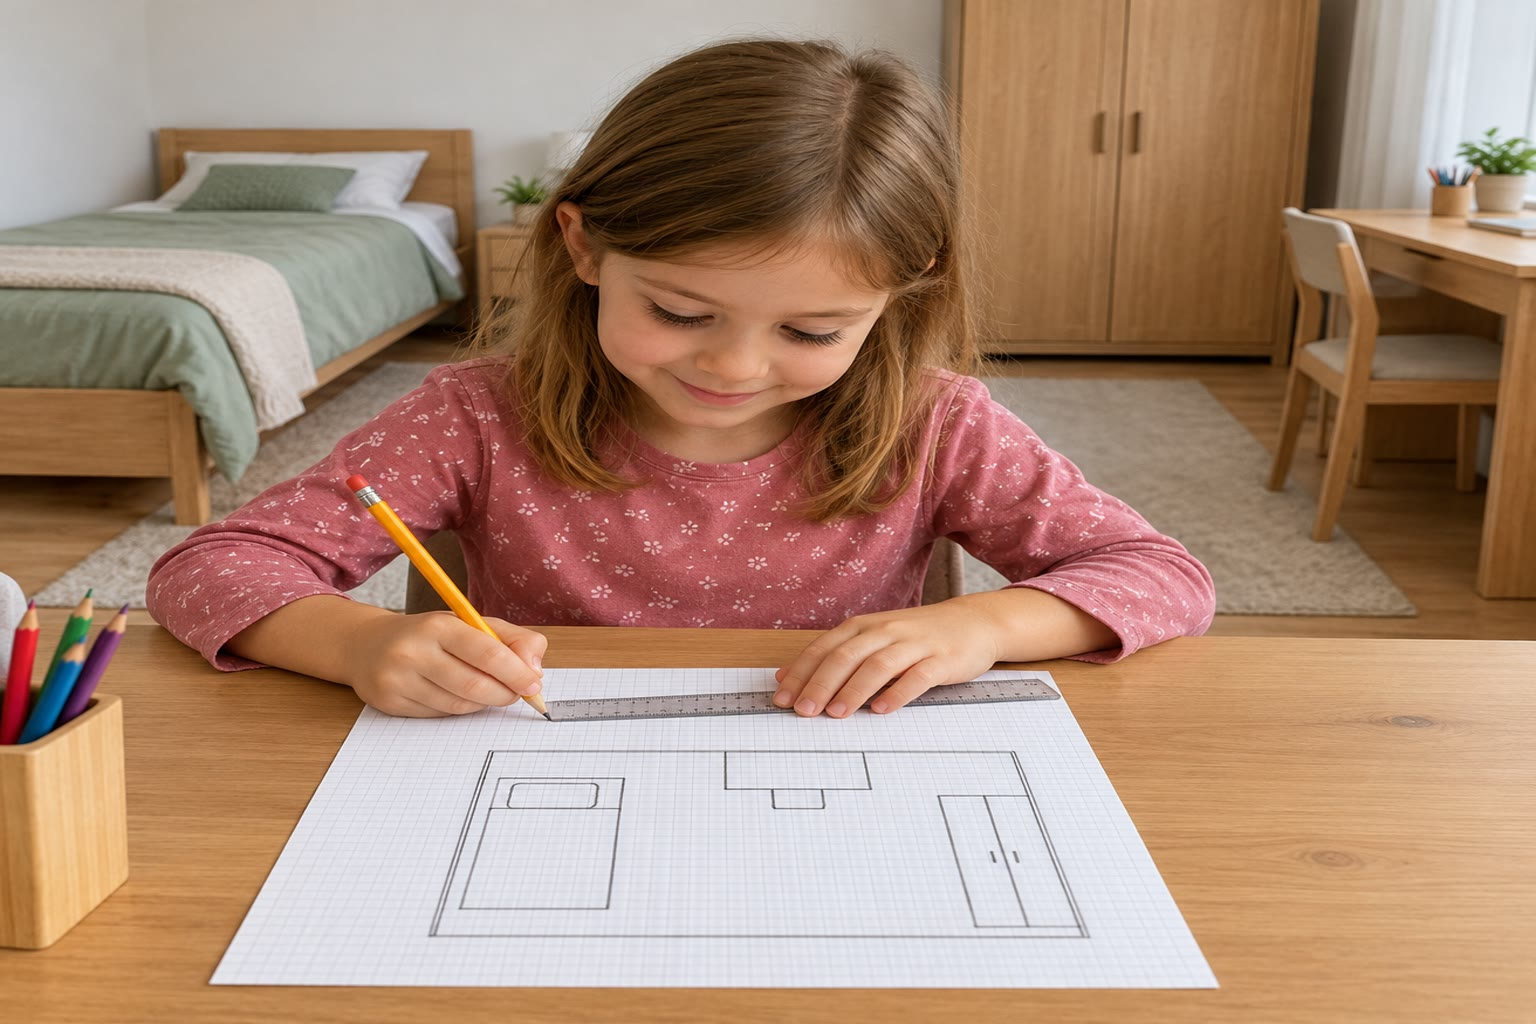
\includegraphics[width=0.55\linewidth]{images/book1/ai/g2-bedroom-plan.jpg}

{\small Desenhando a \omterm{def:g2:drawing-to-map:plan}{planta} de um quarto em papel quadriculado.}
\end{omfigure}

\section{Da planta ao mapa}

Uma \omterm{def:g2:drawing-to-map:plan}{planta} mostra um lugar pequeno. Quando desenhamos um lugar maior ---
uma cidade inteira, um \omterm{def:g1:landscapes-around-us:landform}{vale}, um país ---, desenhamos um \omterm{def:g2:drawing-to-map:map}{mapa}.

\begin{definition}[Mapa]\label{def:g2:drawing-to-map:map}
Um \emph{mapa}\index{mapa} é um desenho de uma grande parte da superfície
da Terra, visto de cima e desenhado muito menor do que é na realidade.
\end{definition}

Num \omterm{def:g2:drawing-to-map:map}{mapa}, uma casa é pequena demais para ser desenhada como é de verdade;
por isso, quem faz \omterm{def:g2:drawing-to-map:map}{mapas} usa sinais pequenos: um ponto para um sítio, uma
linha azul para um \omterm{def:g1:landscapes-around-us:water}{rio}, uma mancha verde para um bosque. O significado de
cada sinal aparece num quadro ao lado do \omterm{def:g2:drawing-to-map:map}{mapa}.

\begin{definition}[Legenda]\label{def:g2:drawing-to-map:legend}
Um \emph{símbolo do mapa}\index{simbolo do mapa@símbolo do mapa} é um sinal pequeno que representa um
tipo de coisa numa \omterm{def:g2:drawing-to-map:plan}{planta} ou num \omterm{def:g2:drawing-to-map:map}{mapa}. A \emph{legenda}\index{legenda} é o quadro
que mostra cada símbolo do \omterm{def:g2:drawing-to-map:map}{mapa} com o seu significado.
\end{definition}

\section{Encontrar o caminho: as quatro direções e a rosa dos ventos}

Para dizer onde uma coisa está, ``à esquerda'' ou ``à direita'' não
basta: o que está à sua esquerda está à direita de alguém que está de
frente para você. As pessoas usam quatro direções que são as mesmas para
todo mundo: norte, leste, sul e oeste. Você já as viu nos livros de física,
com a bússola. De manhã o Sol nasce no leste, e à tarde ele se põe no oeste;
o norte e o sul ficam no meio do caminho entre os dois, um em frente ao outro.

\begin{omfigure}
\begin{tikzpicture}[font=\small]
  \pic[scale=1.5, transform shape] at (0,0) {compassrose};
  \node[align=left, anchor=west, font=\small] at (2.6,0.3)
    {N = norte (no alto da maioria dos mapas)\\L = leste (à direita)\\S = sul (embaixo)\\O = oeste (à esquerda)};
\end{tikzpicture}

{\small Uma \omterm{def:g2:drawing-to-map:directions}{rosa dos ventos}. Entre o norte e o leste fica o nordeste; entre o
sul e o oeste, o sudoeste.}
\label{fig:g2:drawing-to-map:rose}
\end{omfigure}

\begin{definition}[Rosa dos ventos]\label{def:g2:drawing-to-map:directions}
A \emph{rosa dos ventos}\index{rosa dos ventos} é a estrela desenhada num \omterm{def:g2:drawing-to-map:map}{mapa}
que mostra as direções norte, leste, sul e oeste. Na maioria dos \omterm{def:g2:drawing-to-map:map}{mapas}, o
norte fica no alto, o leste à direita, o sul embaixo e o oeste à esquerda.
\end{definition}

\begin{safety}
Nunca olhe para o Sol para achar o leste ou o oeste: isso pode machucar os
seus olhos para sempre. Olhe as sombras, ou use uma bússola.
\end{safety}

\section{Ler um mapa de verdade}

Todo bom \omterm{def:g2:drawing-to-map:map}{mapa} tem quatro partes: um \textbf{título} que diz o que o \omterm{def:g2:drawing-to-map:map}{mapa}
mostra, uma \textbf{\omterm{def:g2:drawing-to-map:legend}{legenda}}, uma \textbf{\omterm{def:g2:drawing-to-map:scale}{escala}} e uma \textbf{\omterm{def:g2:drawing-to-map:directions}{rosa dos
ventos}} (ou pelo menos uma seta que aponta para o norte). Este é o \omterm{def:g2:drawing-to-map:map}{mapa} de
um \omterm{def:g1:landscapes-around-us:landform}{vale} entre \omterm{def:g1:landscapes-around-us:landform}{colinas}, as Colinas de Varden. É o \omterm{def:g1:landscapes-around-us:landform}{vale} inventado que você vai
reencontrar muitas vezes neste livro e nos próximos, cada vez desenhado
com mais detalhes.

\begin{omfigure}
\begin{tikzpicture}
\begin{axis}[width=9.6cm, scale only axis,
    xmin=0, xmax=10, ymin=0, ymax=8, axis equal image,
    xtick={0,...,10}, ytick={0,...,8}, xticklabels={}, yticklabels={},
    grid=major, grid style={black!20}, major tick length=0pt,
    axis background/.style={fill=green!12!omLithAlluv},
    title={\textbf{As Colinas de Varden}}]
  \addplot[fill=omHypsLandD, draw=omHypsLandE!80!black, line width=0.4pt, fill opacity=0.85,
    unbounded coords=jump, even odd rule] table {figdata/out/grade-2-varden_plan-hills.dat};
  \addplot[fill=green!45!black!55, draw=green!35!black, line width=0.4pt] table {figdata/out/grade-2-varden_plan-wood.dat};
  \addplot[ocBlue!85!black, line width=2.2pt] table {figdata/out/shared-region-river.dat};
  \addplot[red!65!black, line width=1.3pt] table {figdata/out/grade-2-varden_plan-road.dat};
  \fill[black] (axis cs:5.012,3.414) ++(-3pt,-4pt) rectangle ++(6pt,8pt);
  \fill[white] (axis cs:5.012,3.414) ++(-1.6pt,-4pt) rectangle ++(3.2pt,8pt);
  \fill[brown!70!black] (axis cs:2.5,3.5) ++(-3.5pt,-3.5pt) rectangle ++(7pt,7pt);
  \fill[red!70!black] (axis cs:7.5,5.5) ++(-5pt,-3pt) rectangle ++(4pt,4pt);
  \fill[red!70!black] (axis cs:7.5,5.5) ++(1pt,-3pt) rectangle ++(4pt,4pt);
  \fill[red!70!black] (axis cs:7.5,5.5) ++(-2pt,2pt) rectangle ++(4pt,4pt);
\end{axis}
\begin{scope}[shift={(10.2,6.4)}, font=\small]
  \node[anchor=west, font=\small\bfseries] at (-0.1,0.55) {Legenda};
  \fill[omHypsLandD, draw=omHypsLandE!80!black] (0,-0.2) rectangle (0.7,0.15); \node[anchor=west] at (0.85,0) {colinas};
  \fill[green!45!black!55] (0,-0.85) rectangle (0.7,-0.5); \node[anchor=west] at (0.85,-0.67) {bosque};
  \draw[ocBlue!85!black, line width=2.2pt] (0,-1.35) -- (0.7,-1.35); \node[anchor=west] at (0.85,-1.35) {rio};
  \draw[red!65!black, line width=1.3pt] (0,-2.0) -- (0.7,-2.0); \node[anchor=west] at (0.85,-2.0) {estrada};
  \fill[black] (0.25,-2.8) rectangle (0.45,-2.5); \fill[white] (0.3,-2.8) rectangle (0.4,-2.5); \node[anchor=west] at (0.85,-2.65) {ponte};
  \fill[brown!70!black] (0.23,-3.45) rectangle (0.47,-3.21); \node[anchor=west] at (0.85,-3.33) {sítio};
  \foreach \dx/\dy in {0.12/-4.1, 0.33/-4.1, 0.22/-3.92}
    \fill[red!70!black] (\dx,\dy) rectangle ++(0.13,0.13);
  \node[anchor=west] at (0.85,-3.98) {vila};
  \draw[black!40] (0,-4.95) rectangle (0.5,-4.45); \node[anchor=west, align=left] at (0.85,-4.7) {1 quadradinho\\= 1 quilômetro};
  \pic[scale=0.75, transform shape] at (0.8,-6.5) {compassrose};
\end{scope}
\end{tikzpicture}

{\small Um \omterm{def:g2:drawing-to-map:map}{mapa} simples das Colinas de Varden, com o título, a \omterm{def:g2:drawing-to-map:legend}{legenda}, a \omterm{def:g2:drawing-to-map:scale}{escala}
e a \omterm{def:g2:drawing-to-map:directions}{rosa dos ventos}. O \omterm{def:g1:landscapes-around-us:water}{rio} corre de oeste para leste.}
\label{fig:g2:drawing-to-map:varden}
\end{omfigure}
% (figdata/grade-2/varden_plan.py; the region: figdata/shared/region.py)

\begin{method}[Ler um mapa]\label{met:g2:drawing-to-map:read}
\begin{enumerate}
  \item Leia o título: que lugar o \omterm{def:g2:drawing-to-map:map}{mapa} mostra?
  \item Leia a \omterm{def:g2:drawing-to-map:legend}{legenda}: o que significa cada símbolo?
  \item Encontre a \omterm{def:g2:drawing-to-map:directions}{rosa dos ventos}: onde fica o norte?
  \item Leia a \omterm{def:g2:drawing-to-map:scale}{escala} e conte os quadradinhos para achar as distâncias.
\end{enumerate}
\end{method}

\begin{example}[Do sítio até a vila]\label{ex:g2:drawing-to-map:farm}
No \omterm{def:g2:drawing-to-map:map}{mapa} das Colinas de Varden, o sítio fica ao sul do \omterm{def:g1:landscapes-around-us:water}{rio}. Para ir até a vila,
o sitiante pega a estrada para o leste, atravessa o \omterm{def:g1:landscapes-around-us:water}{rio} pela ponte e
continua para o nordeste. A vila fica 5 quadradinhos a leste do sítio e 2
quadradinhos ao norte dele: isso dá 5 quilômetros para o leste e 2
quilômetros para o norte.
\end{example}

\section{Exercícios}

\begin{exercise}[$\star$]\label{exo:g2:drawing-to-map:1}
Uma \omterm{def:g2:drawing-to-map:plan}{planta} é desenhada como vista de lado ou como vista de cima?
\end{exercise}

\begin{exercise}[$\star$]\label{exo:g2:drawing-to-map:2}
Na \omterm{def:g2:drawing-to-map:plan}{planta} da sala de aula, o que está desenhado em azul na parede oeste? O
que há no canto nordeste?
\end{exercise}

\begin{exercise}[$\star$]\label{exo:g2:drawing-to-map:3}
Cite as quatro partes que todo bom \omterm{def:g2:drawing-to-map:map}{mapa} deve ter.
\end{exercise}

\begin{exercise}[$\star$]\label{exo:g2:drawing-to-map:4}
Na maioria dos \omterm{def:g2:drawing-to-map:map}{mapas}, que direção fica no alto? E qual fica à esquerda?
\end{exercise}

\begin{exercise}[$\star$]\label{exo:g2:drawing-to-map:5}
Na \omterm{def:g2:drawing-to-map:plan}{planta} da sala de aula, uma carteira ocupa 2 quadradinhos por 1
quadradinho. Qual é o comprimento e a largura de uma carteira na sala de verdade?
\end{exercise}

\begin{exercise}[$\star$]\label{exo:g2:drawing-to-map:6}
No \omterm{def:g2:drawing-to-map:map}{mapa} das Colinas de Varden, o que o quadradinho marrom representa? E a
mancha verde?
\end{exercise}

\begin{exercise}[$\star\star$]\label{exo:g2:drawing-to-map:7}
No \omterm{def:g2:drawing-to-map:map}{mapa} das Colinas de Varden, o bosque fica ao norte ou ao sul do \omterm{def:g1:landscapes-around-us:water}{rio}? Fica a
leste ou a oeste do sítio?
\end{exercise}

\begin{exercise}[$\star\star$]\label{exo:g2:drawing-to-map:8}
No \omterm{def:g2:drawing-to-map:map}{mapa} das Colinas de Varden, o \omterm{def:g2:drawing-to-map:map}{mapa} inteiro tem 10 quadradinhos de oeste a
leste e 8 quadradinhos de sul a norte. Quantos quilômetros isso dá em cada
direção?
\end{exercise}

\begin{exercise}[$\star\star$]\label{exo:g2:drawing-to-map:9}
Na \omterm{def:g2:drawing-to-map:plan}{planta} da sala de aula, quantas carteiras há? Um aluno se senta na
carteira mais perto da porta. Ela fica no norte ou no sul da sala?
\end{exercise}

\begin{exercise}[$\star\star$]\label{exo:g2:drawing-to-map:10}
Lucas desenha a \omterm{def:g2:drawing-to-map:plan}{planta} do seu quarto. A cama dele tem 2 metros de
comprimento. Com a \omterm{def:g2:drawing-to-map:scale}{escala} ``1 quadradinho representa 1 metro'', quantos
quadradinhos de comprimento a cama tem na \omterm{def:g2:drawing-to-map:plan}{planta}? O quarto tem 4 metros de
comprimento e 3 metros de largura: quantos quadradinhos o quarto inteiro ocupa?
\end{exercise}

\begin{exercise}[$\star\star$]\label{exo:g2:drawing-to-map:11}
Lena diz: ``O \omterm{def:g1:landscapes-around-us:water}{rio} está à minha esquerda.'' Por que isso não nos diz onde
o \omterm{def:g1:landscapes-around-us:water}{rio} está? Diga a mesma coisa de um jeito que valha para todo mundo, se
ela estiver no sítio das Colinas de Varden.
\end{exercise}
